\documentclass[10pt,landscape]{article}
\usepackage{multicol}
\usepackage{calc}
\usepackage{ifthen}
\usepackage[landscape]{geometry}
\usepackage{hyperref}

\usepackage[OT1]{fontenc}
\usepackage[sc]{mathpazo}
\usepackage[utf8]{inputenc}
\usepackage[german]{babel}
\usepackage{amsmath}
\usepackage{amsfonts}
\usepackage{amssymb}
\usepackage{mathtools}
\usepackage{fancyhdr}
\usepackage{setspace}
\usepackage{listings}
\usepackage{stmaryrd}
\usepackage{graphicx}
\usepackage{changepage}
\usepackage{enumitem}
\usepackage{wrapfig}
\usepackage{tikz} 
\usepackage{xcolor, soul}
\newcommand{\green}[1]{\sethlcolor{green}\hl{#1}}
\newcommand{\yellow}[1]{\sethlcolor{yellow} \hl{#1}}
\newcommand{\blue}[1]{\sethlcolor{cyan} \hl{#1}}


% To make this come out properly in landscape mode, do one of the following
% 1.
%  pdflatex latexsheet.tex
%
% 2.
%  latex latexsheet.tex
%  dvips -P pdf  -t landscape latexsheet.dvi
%  ps2pdf latexsheet.ps


% If you're reading this, be prepared for confusion.  Making this was
% a learning experience for me, and it shows.  Much of the placement
% was hacked in; if you make it better, let me know...


% 2008-04
% Changed page margin code to use the geometry package. Also added code for
% conditional page margins, depending on paper size. Thanks to Uwe Ziegenhagen
% for the suggestions.

% 2006-08
% Made changes based on suggestions from Gene Cooperman. <gene at ccs.neu.edu>


% To Do:
% \listoffigures \listoftables
% \setcounter{secnumdepth}{0}


% This sets page margins to .5 inch if using letter paper, and to 1cm
% if using A4 paper. (This probably isn't strictly necessary.)
% If using another size paper, use default 1cm margins.
\ifthenelse{\lengthtest { \paperwidth = 11in}}
	{ \geometry{top=.5in,left=.5in,right=.5in,bottom=.5in} }
	{\ifthenelse{ \lengthtest{ \paperwidth = 297mm}}
		{\geometry{top=1cm,left=1cm,right=1cm,bottom=1cm} }
		{\geometry{top=1cm,left=1cm,right=1cm,bottom=1cm} }
	}

% Turn off header and footer
\setcounter{page}{1}


% Redefine section commands to use less space
\makeatletter
\renewcommand{\section}{\@startsection{section}{1}{0mm}%
                                {-1ex plus -.5ex minus -.2ex}%
                                {0.5ex plus .2ex}%x
                                {\normalfont\large\bfseries}}
\renewcommand{\subsection}{\@startsection{subsection}{2}{0mm}%
                                {-1explus -.5ex minus -.2ex}%
                                {0.5ex plus .2ex}%
                                {\normalfont\normalsize\bfseries}}
\renewcommand{\subsubsection}{\@startsection{subsubsection}{3}{0mm}%
                                {-1ex plus -.5ex minus -.2ex}%
                                {1ex plus .2ex}%
                                {\normalfont\small\bfseries}}
\makeatother

% Define BibTeX command
\def\BibTeX{{\rm B\kern-.05em{\sc i\kern-.025em b}\kern-.08em
    T\kern-.1667em\lower.7ex\hbox{E}\kern-.125emX}}

% Don't print section numbers
\setcounter{secnumdepth}{0}


\setlength{\parindent}{0pt}
\setlength{\parskip}{0pt plus 0.5ex}


% -----------------------------------------------------------------------

\begin{document}
\raggedright
\footnotesize
\begin{multicols}{3}


% multicol parameters
% These lengths are set only within the two main columns
%\setlength{\columnseprule}{0.25pt}
\setlength{\premulticols}{1pt}
\setlength{\postmulticols}{1pt}
\setlength{\multicolsep}{1pt}
\setlength{\columnsep}{2pt}

\begin{center}
     \Large{\textbf{Compiler Design - Cheatsheet}} \\
\end{center}
\section{Compiler Structure}
\subsection{Simplified Compiler Structure}

\begin{align*}
    &\text{Source Code} \rightarrow \\
    &\underbrace{\text{Lexical Analysis}\rightarrow^{\text{Token Stream}} \text{Parsing}
    \rightarrow^{\text{Abstract Syntax Tree}}}_{\text{Front End}} \\
    &\underbrace{\text{Intermediate Code Generation} \rightarrow^{\text{Intermediate Code}}}_{\text{Middle End}} \\
    &\underbrace{\text{Code Generation}}_{\text{Back End}}
\end{align*}
\subsection{Stack layout}
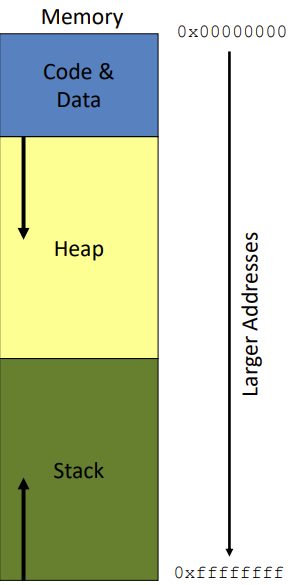
\includegraphics[width = 0.1\textwidth]{Bilder/stack.png}
\subsection{Suffiexes}
\begin{enumerate}
    \item  q = quadword (4 words)
    \item l = long (2 words)
    \item w = word (16-bit)
    \item b = byte (8-bit) 
\end{enumerate}
\subsection{movq-instruction}
movq $SRC$, $DST$ = $DST \leftarrow SRC$ \\
\subsection{Flags}
\begin{center}
    \begin{tabular}{|c|c|} 
     \hline
     e (equality) & ZF is set \\ \hline
     ne (inequality) & (not ZF) \\ \hline
     g (greater than) & (not ZF) and (SF $=$ OF)  \\ \hline
     l (less than) & SF $<>$ OF\\ \hline
     ge (greater or equal) & (SF $=$ OF)  \\ \hline
     e (less than or equal) & SF $<>$ OF or Z  \\ \hline  
    \end{tabular}
  \end{center}
\subsection{Addressing}
\begin{center}
    \begin{tabular}{|c|c|} 
     \hline
     $-8$ ($\%$rsp) & rsp $–$ 8 \\ \hline
     ($\%$rax, $\%$rcx) & rax $+$ 8$\cdot$rcx \\ \hline
     8($\%$rax, $\%$rcx) & rax $+$ 8$\cdot$rcx + 8  \\ \hline
    \end{tabular}
  \end{center}
\subsection{leaq vs. movq}
In leaq we just compute the address, in movq we dereference the address. \\
\subsection{Callee vs. Caller saved}
Caller saved register (Rdi, Rsi, Rdx, Rcx, R09, R08, Rax, R10, R11) are saved by the caller befor calling the function. Callee saved register 
(Rbx, R12, R13, R14, R15) are saved by the called function. \\
\subsection{Parameter} 
\begin{enumerate}
    \item $1 \dots 6$: rdi, rsi, rdx, rcx, r8, r9
    \item $7+$: on the stack (in right-to-left order), nth arg. $((n-7)+2) \cdot 8 + rbp$
\end{enumerate}
\subsection{Why Intermediate Representations?}
\begin{enumerate}
    \item resulting code quality is poor (direct translation)
    \item Richer source language features are hard to encode (Structured data types, Objects, \dots)
    \item hard to optimize
    \item Control-flow is not structured
\end{enumerate}
\subsection{Basic Blocks}
\begin{enumerate}
    \item Starts with a label that names the entry point of the basic block
    \item Ends with a control-flow instruction
    \item Contains no other control-flow instructions
    \item Contains no interior label used as a jump target
\end{enumerate}
\subsection{CFGs}
\begin{enumerate}
    \item Nodes are basic blocks
    \item There is a directed edge from node A to node B if the control flow
    instruction at the end of block A might jump to the label of block B
    \item No two blocks have the same label
\end{enumerate}
\subsection{getelementptr instruction}
The first argument is always a type used as the basis for the calculations. 
The second argument is always a pointer or a vector of pointers, 
and is the base address to start from. The remaining arguments are indices 
that indicate which of the elements of the aggregate object are indexed.
\yellow{GEP never dereferences the address it's calculating}.
\begin{verbatim}
struct RT {
  char A;
  int B[10][20];
  char C;
};
struct ST {
  int X;
  double Y;
  struct RT Z;
};

int *foo(struct ST *s) {
  return &s[1].Z.B[5][13];
}
\end{verbatim} 
is translated in:
\begin{verbatim}
    %arrayidx = getelementptr %struct.ST, ptr %s, i64 1, 
    i32 2, i32 1, i64 5, i64 13
    ret ptr %arrayidx
\end{verbatim}
\subsection*{Regular Expressions}
Regular expressions precisely describe sets of strings. A regular expression R has one of the following forms:
\begin{enumerate}
  \item $\epsilon$: Epsilon stands for the empty string
  \item $'a'$: An ordinary character stands for itself
  \item $R_1 | R_2$: Alternatives, stands for choice of $R_1$ or $R_2$
  \item $R_1 R_2$: Concatenation, stands for $R_1$ followed by $R_2$
  \item $R^*$: Kleene star, stands for zero or more repetitions of $R$
\end{enumerate}
Useful extensions:
\begin{enumerate}
  \item "$foo$": Strings, equivalent to $'f'$ $'o'$ $'o'$
  \item $R^+$: One or more repetitions of $R$, equivalent to $RR^*$
  \item $R$?: Zero or one occurrences of $R$, equivalent to $(\epsilon|R)$
  \item $['a'-'z']$: One of $a$ or $b$ or $c$ or \dots $z$, equivalent to $(a|b|\dots|z)$
  \item $[\text{ }\Hat{ }\text{  }'0'-'9']$: Any character except $0$ through $9$
  \item $R$ as $x$: Name the string matched by $R$ as $x$
\end{enumerate}
\subsection{Chomsky Hierarchy}
Regular $\subset$ Context-Free $\subset$ Context Sensitive $\subset$ Recursively Enumerable \\
\subsection{Matching Rule for Lexer}
Most languages choose “longest match”.
\subsection{Lexer Generator}
\begin{enumerate}
  \item Reads a list of regular expressions: $R_1,\dots,R_n$ , one per token
  \item Each token has an attached “action” $A_i$ (just a piece of code to run
  when the regular expression is matched)  
\end{enumerate}
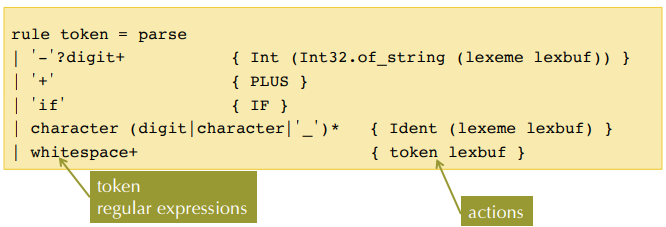
\includegraphics[width = 0.3\textwidth]{Bilder/lexer_generator.png}
Generates scanning code that:
\begin{enumerate}
  \item Decides whether the input is of the form $(R_1|\dots|R_n)^*$
  \item After matching a (longest) token, runs the associated action 
\end{enumerate}
\subsection{Implementation Strategies}
We can use a finite automaton since one must exist for a regular expression.
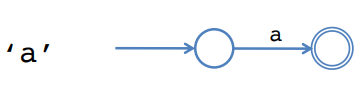
\includegraphics[width = 0.3\textwidth]{Bilder/rule1.png}
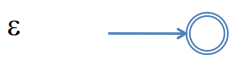
\includegraphics[width = 0.2\textwidth]{Bilder/rule2.png}
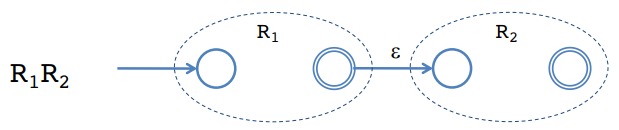
\includegraphics[width = 0.3\textwidth]{Bilder/rule3.png}
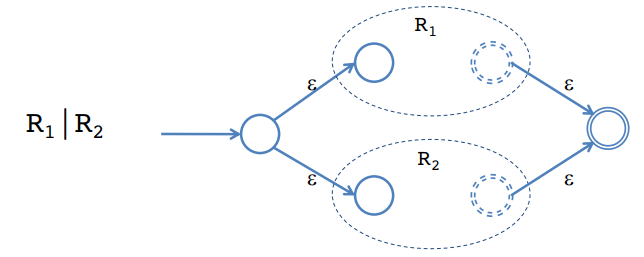
\includegraphics[width = 0.3\textwidth]{Bilder/rule4.png}
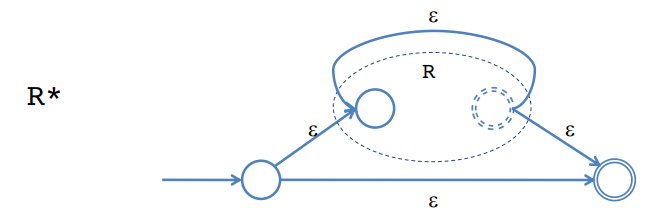
\includegraphics[width = 0.3\textwidth]{Bilder/rule5.png}
\subsection{DFA vs. NFA}
DFA:
\begin{enumerate}
  \item Action of the automaton for each input is fully determined
  \item Accepts if the input is consumed upon reaching an accepting state
  \item Obvious table-based implementation
\end{enumerate}
NFA:
\begin{enumerate}
  \item Automaton potentially has a choice at every step
  \item Accepts an input if there exists a way to reach an accepting state
  \item Less obvious how to implement efficiently
\end{enumerate}
\newpage

\end{multicols}
\end{document}
